\documentclass[../PFC.tex]{subfiles}
\begin{document}

\section{Introducción}
\label{App:Introducción}

Anteriormente se han explicado los conocimientos y términos generales relacionados con la seguridad en la autenticidad NFC basada en criptología con curvas elípticas. A continuación se muestra la aplicación de dichos conocimientos en un proyecto software experimental. El objetivo es demostrar la capacidad de los dispositivos NFC para, de la mano de la criptografía con curvas elípticas, llegar a desarrollar un sistema de autenticación óptimo y fiable.\\

Tanto los nombres, librerías, herramientas, así como el resto del material utilizado se describirán a continuación. A su vez, siguiendo un estándar de desarrollo software basado en metodologías ágiles, se mostrará la utilizada para éste proyecto. Para ello,  el autor y director de este TFG (Fidel Abascal y Domingo Gómez) hemos actuado y ejercido tanto de cliente como de contratado para el desarrollo de la aplicación. \\

Dentro de un ámbito ficticio, una empresa llamada \textbf{Alpha - Consultora S.A.}\footnote{Cualquier similitud con la realidad es mera coincidencia}, nueva potencia local dentro del campo de la seguridad bancaria, que ha cosechado unos excelentes resultados a lo largo de sus 2 años de existencia. Cuenta con más de 40 trabajadores y su crecimiento y expansión es notoria. Tanto es el éxito de esta empresa que, para dar cabida a su plantilla, ha decidido trasladarse a una nueva sede más moderna, amplia y mejor ubicada. La empresa, antes de instalarse en la nueva sede, decide contratar a unos expertos en seguridad para gestionar el control de accesos mediante un sistema de tarjetas y lectores en las entradas; teniendo en cuenta una inversión mínima pero garantizando un alto grado de seguridad. \\

Tras buscar incesantemente recurren a la empresa \textbf{F-NFC}. Una vez realizado el estudio por parte de F-NFC, se pone en consonancia un acuerdo para elaborar una aplicación que genere información que autentifique a un usuario de la empresa \textit{Alpha} y sea reconocido de forma unívoca para permitir su acceso a la sede. La infraestructura de la empresa propietaria de la nueva sede corresponde a la figura \ref{img:infraestructura}.

\label{img:infraestructura}
\begin{figure}[!ht]
  \centering
  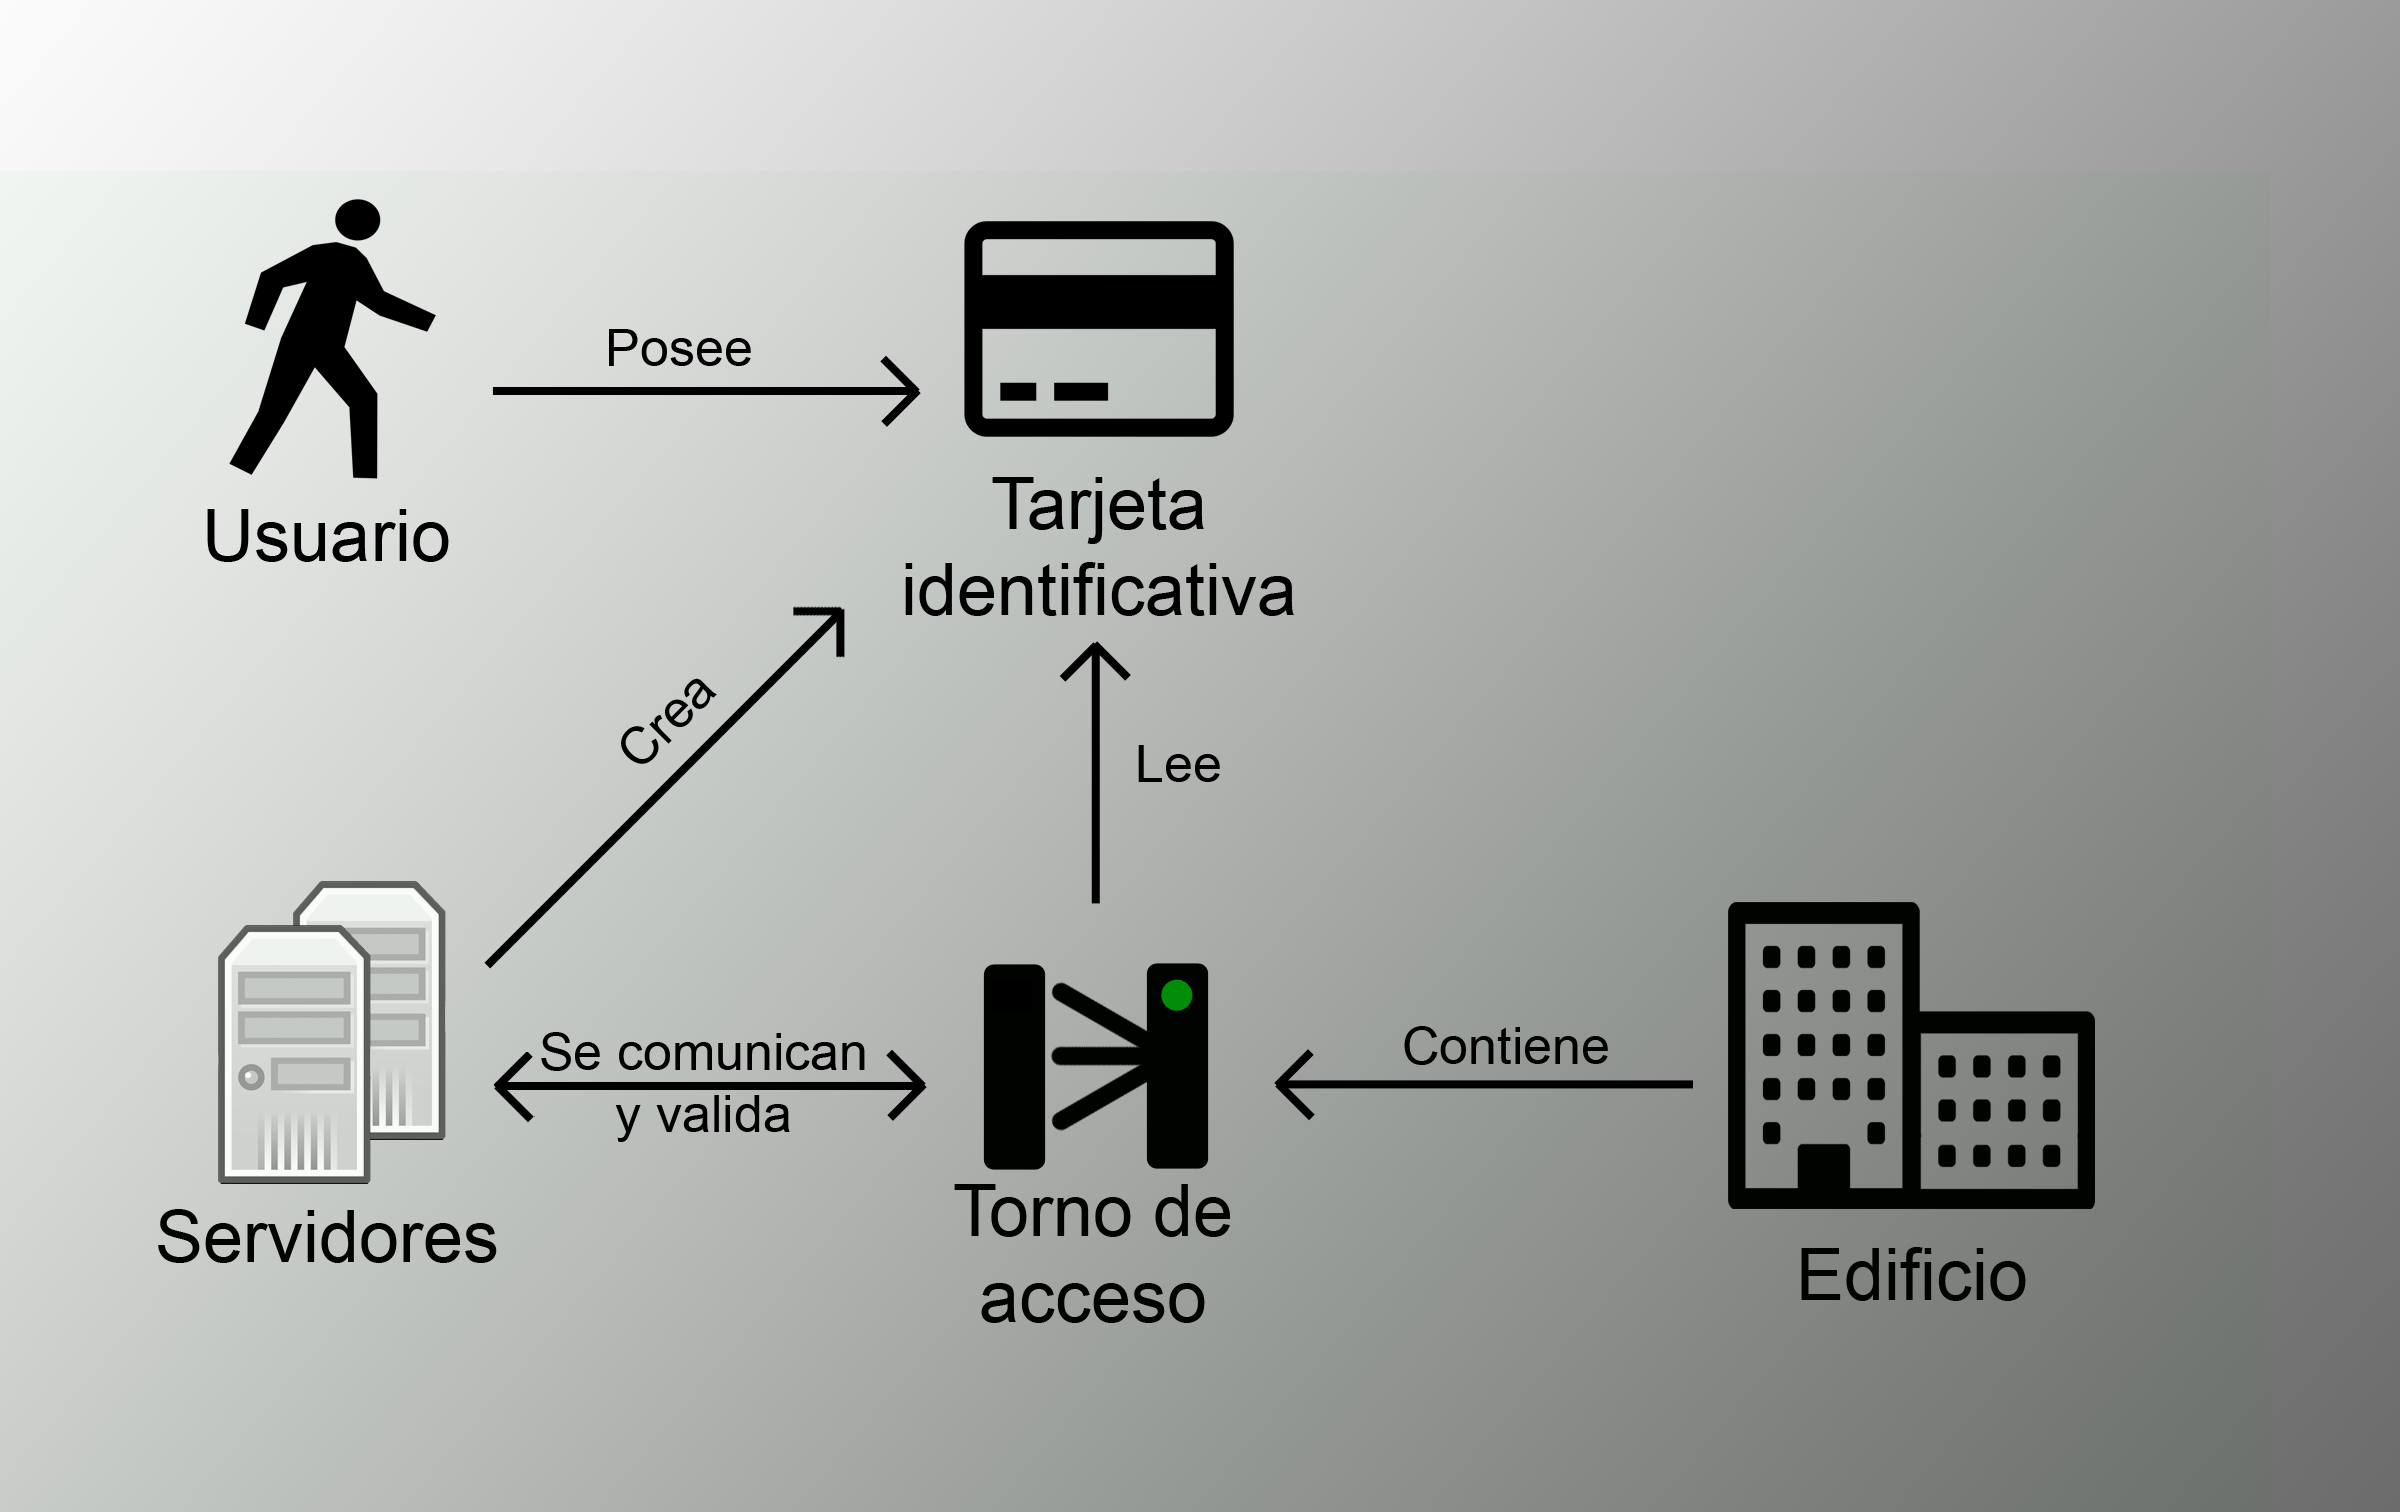
\includegraphics[width=1\textwidth]{./img/arquitecturaVirtual}
  \caption{Infraestructura del sistema ficticio.}
\end{figure}

Los detalles de implementación de la aplicación seguirán un objetivo didáctico y experimental que cumplirán los requerimientos de la situación propuesta; adecuándose a la carencia real de la infraestructura anteriormente mencionada. Se explicará en las secciones siguientes en detalle todos los puntos implicados en la consecución de este objetivo. Más concretamente en el apartado de escenario de la aplicación \ref{App:Escenario}.

\section{Material utilizado}
\label{App:Material utilizado}

Para el desarrollo del proyecto se ha utilizado, ante todo, software de carácter libre junto a imágenes, textos, estructuras y contenido sin restricciones de uso. Ya sea debido al tipo de licencia de cada elemento o por ser de autoría propia.
\\\\
El desarrollo se ha realizado en el lenguaje de programación \textit{Java} con el kit de desarrollo \textit{Java} (JDK) 1.8.65 (\textit{Java 8 update 65}) de \textit{Oracle Corporation}\cite{java}.
\\\\
El entorno de desarrollo integrado o \textit{IDE} de la aplicación es el oficial de Google para el desarrollo para dispositivos \textit{Android}: \textit{Android Studio}, versión 1.5.1\cite{androidStudio}. Este programa provee las herramientas básicas de desarrollo; entre ellas, un administrador de los kit de desarrollo o \textit{SDKs} para las diferentes versiones y varios elementos descritos a continuación: 
\begin{itemize}
\item{Plataformas SDK}
	\begin{itemize}
	\item{API 22: Para la versión Android 5.1.1.}
	\item{API 21: Para la versión Android 5.0.1.}
	\end{itemize}
\item{Herramientas SDK}
	\begin{itemize}
	\item{Android Build Tools : Para la construcción de la aplicación.}
	\item{Android SDK Platform Tools v23.1: Soporte para el desarrollo.}
	\item{Repositorio de ayuda Android, rev 30.}
	\item{Libreria de ayuda Android, rev 23.2.1 : Ayudas en la retrocompatibilidad 	de elementos de interfaz de usuario.}
	\item{Google USB Driver, rev 11 : Conexión entre el servicio de ejecución de la aplicación y los dispositivos USB.}
	\item{Intel x86 HAXM, rev 6.0.1 : Aceleración \textit{hardware} para la emulación.}
	\end{itemize}
\end{itemize}

Estos componentes de \textit{Android Studio} hacen posible el desarrollo de la aplicación objetivo. Este programa, con carencias notorias en ciertos apartados, ha hecho complicado, de cierta forma, la selección de componentes a instalar, versiones y etcétera debido a diversos motivos de compatibilidades de librerías y actualizaciones desfasadas entre los componentes y el propio IDE. 
\\\\
La esencia de la aplicación reside en la criptografía mediante curvas elípticas. Para la implementación de ello ha sido necesario utilizar una librería externa llamada \textit{Bouncy Castle}\cite{bouncyCastle} versión 1.54. Dicha librería suple las deficiencias de la implementación base de la propia API (\textit{Application Programming Interface}) de \textit{Java}. La cual tiene limitaciones claras a la hora de la generar curvas elípticas. Gracias a ésta librería se ha podido realizar la parte crítica de la aplicación con una mejora de rendimiento notoria si hubiera que haber utilizado la API de \textit{Java}. 
\\\\
Respecto al almacenaje de datos se ha optado por utilizar una pequeña base de datos en \textit{SQLite}\cite{sqlite} descrita más adelante. Para el almacenamiento de unos pequeños registros que utilizará la aplicación. El uso de una base de datos de mayor capacidad y funcionalidades no se ha contemplado factible. 
\\\\
En cuanto a los elementos gráficos de la aplicación, un alto porcentaje son de elaboración propia mediante programas de edición de imágenes. El resto son de libre uso comercial. La iconografía de la aplicación es autoría de \textit{Google Inc.}\cite{googleIcons}. Dichos iconos han de ser vectoriales debido a la optimización del tratamiento de imágenes y su renderizado, por lo que en este aspecto, \textit{Google} provee estos  iconos en formato \textit{SVG} y \textit{PNG}; también \textit{Android Studio} de forma nativa pero no actualizada. A la hora de incluir estos elementos externos se ha transformado las descripciones vectoriales \textit{SVG} (\textit{Scalable Vector Graphics}) en formato \textit{XML} (\textit{eXtensible Markup Language}) interpretable de forma sencilla por \textit{Android Studio}. En el apartado de diseño y aspecto de la aplicación \ref{App:Diseño y aspecto} se comenta en detalle el resto de la disposición, motivación y elaboración gráfica de la aplicación. 
\\\\
La API de objetivo del proyecto \textit{Android} ha sido la número 22. Desarrollada para la versión 5.1. (\textit{LOLLIPOP MR1}). Se ha decidido utilizar esta esta API debido a las mejoras sustanciales en cuanto al trabajo del adaptador NFC implementadas desde la versión 5.0\cite{androidAPI21} y mejoradas en ésta\cite{androidAPI22}. 
\\\\
Para el testado de la aplicación \textit{Android Studio} dispone de la tecnología \textit{AVD} para la virtualización de dispositivos \textit{Android}. Sin embargo, el rendimiento es pobre en comparación con el testeo y \textit{debug} en un dispositivo físico. Por lo que se ha utilizado un dispositivo \textit{Android} \textit{smartphone} \textit{One Plus One} de la compañía americana \textit{Never Settle}, el cuál dispone de la versión \textit{Android} 5.1.1 y \textit{Cyanogen OS} 12.1.1  en el momento de la elaboración de la aplicación. 

\label{img:opo}
\begin{figure}[H]
  \centering
  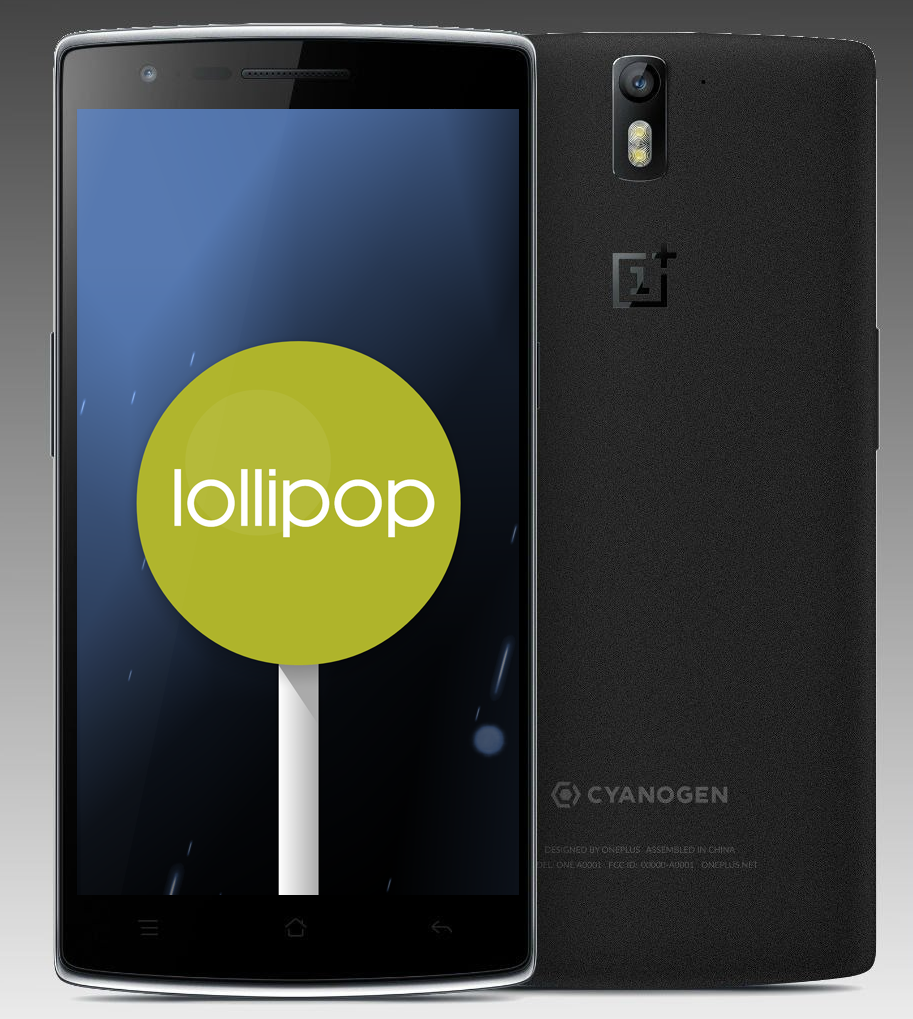
\includegraphics[width=0.4\textwidth]{./img/opo}
  \caption{Smartphone One Plus One - Never Settle}
\end{figure} 

Por último, el proyecto ha necesitado de dos elementos físicos principales: el dispositivo \textit{Android} mencionado anteriormente y de tarjetas NFC. Debido a la carencia de un presupuesto, se ha optado por utilizar etiquetas adesibles (desde ahora NFC-T) de bajo coste por etiqueta. Se trata del chip \textit{NTAG213} que siguen el estándar ISO 14443-3\cite{iso14443}. Las características de estas etiquetas son las siguientes:

\begin{itemize}
\item{Tipo de etiqueta : ISO 14443-3A }
\item{Descripción : NXP MIFARE Ultralight (Ultralight C) - NTAG213}
\item{Tecnología : NfcA, Ndef, MifareUltralight}
\item{Formato de datos: NFC Forum Type 2}
\item{Diámetro: 25 mm}
\item{Identificadores del chip}
	\begin{itemize}
	\item{Valor ATQA: 0x0044}
	\item{Valor SAK: 0x00}
	\item{Firma: NXP Public Key}
	\end{itemize}
\item{Tamaños y capacidad}
	\begin{itemize}
	\item{Memoria: 45 páginas de 4bytes por página (180 bytes)}
	\item{Tamaño: 137 bytes}
	\item{\textit{UID} (Identificador del contenido): 7 bytes\cite{nfcSpecifications}}
		\begin{itemize}
		\item{\textit{Byte 7}: Valor \textit{UTF-8}, codificación}
		\item{\textit{Byte 6}: Valor \textit{0}, reservado para uso futuro}
		\item{\textit{Byte 5-0}: Tamaño del código del lenguaje \textit{IANA}}
		\end{itemize}	
	\item{Tamaño utilizable: 130 bytes (Tamaño menos \textit{UID})}	
	\end{itemize}
\end{itemize}

Estas etiquetas se pueden adherir en una superficie que le haga de soporte. Por ejemplo, se podría plastificar junto a dos tapas que cubran el chip y tener la apariencia de una tarjeta común. Su apariencia es la siguiente: 

\label{img:nfctag}
\begin{figure}[H]
  \centering
  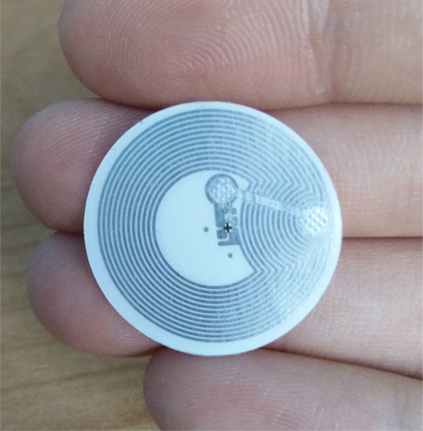
\includegraphics[width=0.5\textwidth]{./img/nfctag}
  \caption{NFC Tag - NTAG213}
\end{figure}

Hubiera sido preferible utilizar chips \textit{MIFARE}\cite{mifare} de alta capacidad y mayores funcionalidades como los \textit{MIFARE classic} 1K y 4K del productor \textit{NXP}. Estos chips están implementados en una enorme cantidad de aplicaciones en todo el mundo, un ejemplo claro de su uso son el de las tarjetas de crédito y la mayoría de chips NFC actuales que impliquen la necesidad de encriptación (RSA comúnmente) y seguridad. En estas tarjetas es realmente complicado acceder a su contenido ya que se precisan ciertas claves para la lectura y decodificación. Sin embargo, en las utilizadas en este proyecto se escribe en texto plano (siguiendo el objetivo didáctico); en el apartado de seguridad y criptología \ref{App:Seguridad y criptología} se explica cómo afectaría esta carencia al sistema final. 
\\\\
Todos los elementos descritos en este apartado conforman lo necesario para simular la estructura descrita en la figura \ref{img:infraestructura} y la implementada definida en el apartado \ref{App:Escenario}. 
\\\\

\section{Metodología}
\label{App:Metodología}

Metodología ágil basada en iteracciones continuas debido a la comunicación continua con el cliente...

Diagrama gantz
\label{img:nfctag}
\begin{figure}[H]
  \centering
  %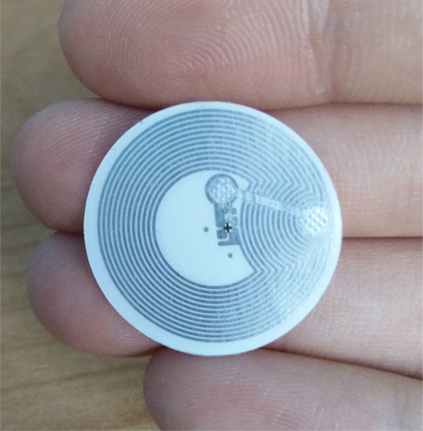
\includegraphics[width=0.5\textwidth]{./img/nfctag}
  \caption{Diagrama Gantt - Subdivisión de elementos de la aplicación para su desarrollo}
\end{figure}

\section{Escenario}
\label{App:Escenario}

La idea principal del escenario de la aplicación se ha comentado en el aparatado \ref{App:Introducción}, en donde se comenta que el objetivo de la aplicación es meramente didáctico y experimental. Alejándose de los modelos pragmáticos del desarrollo profesional. 
\\\\
La complejidad añadida de implementar un sistema cercano a la realidad aplicaría un coste elevado de recursos sin tener relevancia notoria en la finalidad comentada. Elementos tales como: servidores, \textit{WebServices}, \textit{frameworks} de desarrollo, certificación, optimización, etcétera. Dado que la esencia de este TFG se centra en el elemento teórico y didáctico de la criptología en curvas elípticas, la creación de una aplicación de carácter altamente profesional le añadiría beneficios nimios. Los cuales no compensan la complejidad agregada, por lo que se han realizado labores de simulación y descarte de las partes que se han considerado prescindibles.
\\\\
La arquitectura de la aplicación representada en la figura \ref{img:infraestructura} muestra un escenario típico que da pie a la implementación de este tipo de seguridad. Dentro de este proyecto virtual se dispone de un edificio el cuál posee tornos o puertas de acceso. Estas puertas son capaces de leer el contenido de las tarjetas NFC de cada usuario del sistema. El contenido de las tarjetas se transmite a los servidores de validación de la empresa (sin la necesidad de que se encuentren físicamente dentro del mismo edificio). Los servidores validarán la información recogida en el torno de acceso y validará o no el contenido. Si resulta validado el torno recogerá de los servidores la nueva información a escribir en la tarjeta para hacer válida el paso la próxima vez. Finalmente, el usuario por medio de ésta tarjeta unipersonal podrá acceder al edificio autenticándose en la entrada.
\\\\
Descrito el escenario virtual, es necesario comentar el que éste proyecto se ha realizado. Contando con los elementos de \ref{App:Material utilizado} se agruparán los funcionalidades del escenario virtual en el dispositivo \textit{Android}. Por lo tanto, no habrá conexiones a servidores externos y toda la estructura se compondrá únicamente del dispositivo \textit{Android} y las tarjetas NFC. A su vez, contará con las siguientes funciones que simulan labores del escenario virtual:

\begin{itemize}
\item{Información sobre los usuarios del sistema: En lugar de contar con un acceso a una base de datos que recoja la información, se utiliza una pequeña base de datos dentro del dispositivo que contiene la información básica de los usuarios (identificador y nombre del usuario).}
\item{Información del sistema de encriptación: El dispositivo también contiene la información básica del sistema criptológico implementado (labor de información de servidores).}
\item{Validación: Tras leer el contenido de la tarjeta NFC, denegará o validará la información obtenida (labor de validación y acceso).}
\item{Labores de administración del sistema: El dispositivo será capaz de restaurar los valores por defecto del sistema, junto a la información inicial. También permitirá crear nuevas definiciones del sistema de seguridad. Por último, también asignará usuarios al sistema de seguridad que no se encuentren dentro (labor de creación de tarjetas).}
\end{itemize}

Todos los elementos de información se describen en el apartado \ref{App:Base de datos} sobre la base de datos de la aplicación; y las funcionalidades del sistema dentro del apartado \ref{App:Requisitos y funcionalidades} de requisitos y funcionalidades.

\section{Requisitos y funcionalidades}
\label{App:Requisitos y funcionalidades}

La toma de requisitos, especificaciones y funcionalidades de la aplicación real, que cumple con los simulados en el contexto virtual descrito en la introducción \ref{App:Introducción}, se ha llevado a cabo mediante constantes reuniones. 
\\\\
Siguiendo la metodología ágil basada en iteracciones comentada en el apartado \ref{App:Metodología}, desde el primer momento se ha ido mostrando el avance del proyecto al supuesto cliente. Éste ha validado según sus requerimientos iniciales o ha concretado cambios que se adecuen en el marco de las funcionalidades principales.  Iteracción a iteracción se ha ido implementando los pasos siguiendo hitos a validar. El diagrama \textit{Gantt} mostrado en la figura \ref{img:diagramaGantt} muestra en detalle la división de las tareas y apartados del proyecto realizado en este TFG.

Los casos de uso de la aplicación se muestran a continuación :

--

\section{Diseño y aspecto}
\label{App:Diseño y aspecto}

iconografía vectorial\cite{googleIcons}
Material design
intento de material desing (iconos, sombras, disposición de elementos, etcétera
Colores que dan seguridad

\section{Seguridad y criptología}
\label{App:Seguridad y criptología}

hablar de qué ocurre al tener texto plano en las nfc-t en vez de las mifare classic

\section{Base de datos}
\label{App:Base de datos}

Tablas, contenido por defecto.




\end{document}
